\documentclass{beamer}

% --- THEME AND APPEARANCE ---
\usetheme{Madrid} % A clean, popular theme with navigation
\usecolortheme{default}

% --- PACKAGE IMPORTS ---
\usepackage[utf8]{inputenc}
\usepackage{amsmath}     % For advanced math typesetting (e.g., P(A))
\usepackage{amssymb}     % For math symbols
\usepackage{booktabs}    % For clean tables (if needed later)
\usepackage{tikz}        % For diagrams (as requested)
\usetikzlibrary{shapes.arrows, positioning, calc} % Common TikZ extras

% --- PRESENTATION METADATA ---
\title[History of Probability]{The Logic of Chance: A History of Probability}
\subtitle{An Introduction to Logic and Risk}
\author{Brendan Shea, PhD}
\institute{Rochester Community and Technical College}
\date{}

\begin{document}

% --- SLIDE 1: TITLE PAGE ---
% This frame uses the metadata defined above to create the title.
% It serves as our first "slide" and setup.
\begin{frame}
  \titlepage
\end{frame}

% --- SLIDE 2: WHAT IS PROBABILITY? ---
\begin{frame}
\frametitle{What is Probability?}

  \begin{itemize}
    \item At its core, probability is the formal study of uncertainty and chance.
    
    \item We use it to assign a numerical value to how likely a specific \textbf{event}, or a particular outcome, is to occur.
    
    \item This creates a logical framework for reasoning in situations that are not completely \textbf{deterministic}, meaning the outcome is not pre-ordained.
    
    % SPECIAL ELEMENT: Nested List
    \item This study generally breaks into two main conceptual types:
    \begin{itemize}
        \item \textbf{Frequency-Type:} How often does it happen over many trials?
        \item \textbf{Belief-Type:} How sure are you that it will happen?
    \end{itemize}
    
  \end{itemize}
\end{frame}

% --- SLIDE 3: WHY STUDY PROBABILITY? ---
\begin{frame}
\frametitle{Why Study Probability?}

  \begin{itemize}
    \item Probability is not just for card games; it is a fundamental tool for decision-making in daily life.
    
    \item It allows us to understand and quantify \textbf{risk}, which is the chance of an undesirable outcome, in fields from medicine to finance.
    
    \item Many modern technologies, including \textbf{artificial intelligence} (AI), are built on probabilistic models to make predictions from incomplete data.
  \end{itemize}

  % SPECIAL ELEMENT: Alert Block
  \begin{alertblock}{A Core Skill for Logic}
    Understanding probability is essential for \textbf{critical thinking}. It helps us evaluate claims, interpret data, and avoid common logical errors in our reasoning.
  \end{alertblock}

\end{frame}

% --- SLIDE 4: THE MATH: THE PROBABILITY SCALE ---
\begin{frame}
\frametitle{The Math: The Probability Scale}

  \begin{itemize}
    \item The probability of any event, which we write as $P(A)$, is always a number between 0 and 1, inclusive.
    
    \item A probability of 0 means the event is \textbf{impossible}.
    \begin{itemize}
        \item Example: $P(\text{rolling a 7 on a 6-sided die}) = 0$.
    \end{itemize}
    
    \item A probability of 1 means the event is \textbf{certain}.
    \begin{itemize}
        \item Example: $P(\text{rolling a number } < 7 \text{ on a 6-sided die}) = 1$.
    \end{itemize}
  \end{itemize}

  % SPECIAL ELEMENT: TikZ Diagram
  \begin{center}
    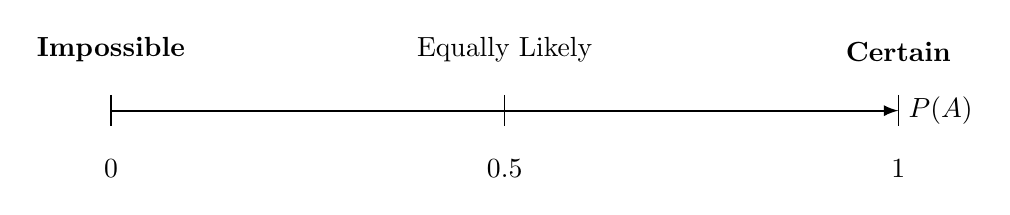
\begin{tikzpicture}[scale=1]
      % Draw the main axis
      \draw [thick, -latex] (0,0) -- (10,0) node[right] {$P(A)$};
      
      % Draw the tick marks
      \draw (0,0.2) -- (0,-0.2) node[below=3mm] {0};
      \draw (5,0.2) -- (5,-0.2) node[below=3mm] {0.5};
      \draw (10,0.2) -- (10,-0.2) node[below=3mm] {1};
      
      % Add labels above the axis
      \node[above=5mm] at (0,0) {\textbf{Impossible}};
      \node[above=5mm] at (5,0) {Equally Likely};
      \node[above=5mm] at (10,0) {\textbf{Certain}};
    \end{tikzpicture}
  \end{center}

\end{frame}

% Continue from the previous document setup...

% --- SLIDE 5: CALCULATING SIMPLE PROBABILITY ---
\begin{frame}
\frametitle{Calculating Simple Probability}

  \begin{itemize}
    \item For events where all outcomes are equally likely, we use a simple ratio to determine probability.
    
    \item The general formula is: $P(A) = \frac{\text{Number of Favorable Outcomes}}{\text{Total Number of Possible Outcomes}}$
    
    \item \textbf{Favorable Outcomes} are the specific results that satisfy the conditions of the event we are interested in.
    
    \item \textbf{Total Outcomes} (or the \textbf{Sample Space}) represents every single possible result.
  \end{itemize}
  
  % SPECIAL ELEMENT: Block
  \begin{block}{Example: Rolling a Die}
    If you roll a standard six-sided die, what is $P(\text{rolling a 4})$? \\
    $P(4) = \frac{1 \text{ (favorable outcome)}}{\text{6 (total outcomes)}} \approx 0.167$
  \end{block}

\end{frame}

% --- SLIDE 6: KEY CONCEPT: SAMPLE SPACE ---
\begin{frame}
\frametitle{Key Concept: Sample Space}

  \begin{itemize}
    \item The **Sample Space** ($\Omega$ or $S$) is the set of all possible outcomes of a random experiment.
    
    \item Defining the Sample Space correctly is the essential first step in any probability calculation.
    
    \item Every event we analyze must be a subset of the complete Sample Space.
    
    \item Changing the experiment changes the Sample Space, which dramatically affects the resulting probabilities.
  \end{itemize}
  
  % SPECIAL ELEMENT: Table for comparison
  \begin{table}
    \centering
    \caption{Defining Sample Spaces}
    \begin{tabular}{ll}
      \toprule
      \textbf{Experiment} & \textbf{Sample Space ($S$)} \\
      \midrule
      Flipping one coin & $\{ \text{Heads, Tails} \}$ \\
      Flipping two coins & $\{ \text{HH, HT, TH, TT} \}$ \\
      Drawing a card & $\{ \text{52 specific cards} \}$ \\
      \bottomrule
    \end{tabular}
  \end{table}

\end{frame}

% --- SLIDE 7: CONCEPT 1: FREQUENCY-TYPE PROBABILITY ---
\begin{frame}
\frametitle{Concept 1: Frequency-Type Probability}

  \begin{itemize}
    \item \textbf{Frequency-Type Probability} (or \textbf{Frequentist Probability}) defines probability based on observation over a large number of trials.
    
    \item It answers the question: "In the long run, how often does this event occur?"
    
    \item The probability is seen as the stable limit of the relative frequency as the number of trials approaches infinity.
    
    \item This type is often used in science, statistics, and quality control where experiments can be repeated many times.
  \end{itemize}
  
  % SPECIAL ELEMENT: Simple List with explanation
  \begin{itemize}
      \item \textbf{Key Idea:} The probability is a characteristic of the physical world, measurable through repetition.
  \end{itemize}

\end{frame}

% --- SLIDE 8: CONCEPT 2: BELIEF-TYPE PROBABILITY ---
\begin{frame}
\frametitle{Concept 2: Belief-Type Probability}

  \begin{itemize}
    \item \textbf{Belief-Type Probability} (or \textbf{Bayesian/Subjective Probability}) defines probability as a degree of belief.
    
    \item It answers the question: "How strongly should a rational person believe this event will occur, given the evidence?"
    
    \item This concept applies to single, non-repeatable events where frequency cannot be measured (e.g., Will a specific historical person win an election?).
    
    \item The probability is relative to the information available to the specific person making the judgment.
  \end{itemize}

  % SPECIAL ELEMENT: Alert Block highlighting the difference
  \begin{alertblock}{Focus on Evidence}
    Belief-type probability explicitly acknowledges that prior knowledge and new evidence must be factored into the final probability assessment. This becomes critical later with Bayes' Theorem.
  \end{alertblock}

\end{frame}

% Continue from the previous document setup...

% --- SLIDE 9: THE BIRTH OF PROBABILITY ---
\begin{frame}
\frametitle{The Birth of Probability: A Gambler's Dispute}

  \begin{itemize}
    \item The formal theory of probability emerged not from an academic pursuit, but from a practical problem: **gambling**.
    
    \item In the 17th century, a French nobleman and passionate gambler, the Chevalier de Méré, posed a famous question.
    
    \item The question involved the "Problem of Points": how should winnings be fairly divided if a game of chance is interrupted early?
    
    \item This dispute required a logical method to calculate the probability of potential future, unplayed rounds.
  \end{itemize}

  % SPECIAL ELEMENT: Alert Block for Context
  \begin{block}{The Problem of Points}
    The dilemma was essentially one of \textbf{expected value}: how much is each side's *chance* worth at the moment the game is stopped?
  \end{block}

\end{frame}

% --- SLIDE 10: MEET THE FOUNDERS ---
\begin{frame}
\frametitle{Meet the Founders: Blaise Pascal \& Pierre de Fermat}

  \begin{itemize}
    \item The Chevalier de Méré presented his gambling problem to the renowned mathematician \textbf{Blaise Pascal} (1623–1662).
    
    \item Pascal, in turn, began corresponding with his contemporary, \textbf{Pierre de Fermat} (1607–1665), about the solution.
    
    \item Their 1654 correspondence became the foundational work that systematically described and solved problems of chance.
    
    \item They established the principle that probability is determined by the ratio of favorable outcomes to all possible outcomes.
  \end{itemize}

  % SPECIAL ELEMENT: Nested List to summarize contributions
  \begin{itemize}
      \item \textbf{Pascal:} Focused on applying combinatorics to solve the problem of points.
      \item \textbf{Fermat:} Independently arrived at the same conclusions using slightly different logical approaches.
  \end{itemize}

\end{frame}

% --- SLIDE 11: CLASSICAL PROBABILITY ---
\begin{frame}
\frametitle{Classical Probability: The "Equally Likely" Principle}

  \begin{itemize}
    \item The **Classical Definition of Probability** (developed by Pascal and others) relies on the principle of indifference.
    
    \item The principle states that if there are $N$ mutually exclusive and exhaustive outcomes, and there is no reason to prefer one over the others, they are all \textbf{equally likely}.
    
    \item This definition is self-contained and logical, but it only applies when all possible outcomes are, in fact, truly symmetrical (like a fair coin or die).
    
    \item This framework is elegant for understanding simple games of chance and forms the basis of combinatorial analysis.
  \end{itemize}

  % SPECIAL ELEMENT: Block with the formula
  \begin{block}{Defining Classical Probability}
    $P(A) = \frac{\text{Number of ways A can occur}}{\text{Total number of outcomes in the Sample Space}}$
  \end{block}

\end{frame}

% Continue from the previous document setup...

% --- SLIDE 12: CLASSICAL PROBABILITY: EXAMPLES (Now Slide 12) ---
\begin{frame}
\frametitle{Classical Probability: Examples in Games of Chance}

  \begin{itemize}
    \item Classical Probability is perfect for scenarios where the \textbf{Sample Space} is known and all outcomes are equally likely.
    
    \item \textbf{Card Games:} The probability of drawing a specific card (e.g., the Ace of Spades) is $1/52$ because there are 52 total outcomes.
    
    \item \textbf{Multiple Events:} The probability of rolling an even number on a six-sided die is $3/6 = 1/2$ (outcomes $\{2, 4, 6\}$).
    
    \item The simplicity of these examples allowed Pascal and Fermat to establish a rigorous mathematical framework.
  \end{itemize}

  % SPECIAL ELEMENT: Nested List with Calculations
  \begin{block}{Calculating Combinations}
    \textbf{Example:} The probability of rolling a total of 7 with two six-sided dice.
    \begin{itemize}
        \item Total Outcomes: $6 \times 6 = 36$
        \item Favorable Outcomes: $\{(1, 6), (2, 5), (3, 4), (4, 3), (5, 2), (6, 1)\} = 6$
        \item $P(\text{total}=7) = \mathbf{6/36} = 1/6 \approx 0.167$
    \end{itemize}
  \end{block}

\end{frame}

% --- SLIDE 13: PHILOSOPHY BREAK: PASCAL'S WAGER (CONCEPT) ---
\begin{frame}
\frametitle{Philosophy Break: Pascal's Wager (The Logic of Infinite Utility)}

  \begin{itemize}
    \item \textbf{Pascal's Wager} uses probability and decision theory to argue for belief in God based on \textbf{expected utility}.
    
    \item The argument is philosophical: the probability that God exists ($P(G)$) is unknown but greater than zero (a \textbf{prior probability}).
    
    \item The potential gain of eternal life is considered \textbf{infinitely large ($\infty$)}, while the loss is finite (a life of piety).
    
    \item According to decision theory, any potential outcome multiplied by infinity yields infinity, making the choice with the infinite payout the most rational.
  \end{itemize}

  % SPECIAL ELEMENT: Block to define the core concept
  \begin{block}{Expected Utility}
    Expected Utility is calculated as: $\sum P(\text{Outcome}) \times \text{Value}(\text{Outcome})$. Pascal argues one side of the ledger is mathematically dominant.
  \end{block}

\end{frame}

% --- SLIDE 14: PASCAL'S WAGER (PAYOFF TABLE) ---
\begin{frame}
\frametitle{Pascal's Wager: The Payoff Table}

  \begin{itemize}
    \item The Wager is best understood as a $2 \times 2$ payoff matrix, comparing the \textbf{actions} (Believe/Don't Believe) against the \textbf{states of the world} (God Exists/God Does Not Exist).
    
    \item The goal is to maximize the payoff, or the utility, of the outcome.
    
    \item The argument hinges on the presence of the $\mathbf{\infty}$ (infinity) sign in the belief column, which dominates the finite payoffs in the non-belief column.
    
    \item This table illustrates how even a small chance of infinite gain outweighs a certain chance of a finite gain or loss.
  \end{itemize}

  % SPECIAL ELEMENT: Payoff Table
  \begin{table}
    \centering
    \caption{The Payoffs of Belief}
    \begin{tabular}{lcc}
      \toprule
      \textbf{Your Action} & \textbf{State: God Exists} & \textbf{State: God Does Not Exist} \\
      \midrule
      \textbf{Believe} & Eternal Gain ($\mathbf{\infty}$) & Finite Loss (e.g., missed pleasure) \\
      \textbf{Don't Believe} & Eternal Loss ($\mathbf{-\infty}$) & Finite Gain (e.g., earthly pleasure) \\
      \bottomrule
    \end{tabular}
  \end{table}

\end{frame}

% --- SLIDE 15: DISCUSSION: OBJECTIONS TO PASCAL'S WAGER (Revised to focus on questions) ---
\begin{frame}
\frametitle{Discussion: Objections to Pascal's Wager}

  \begin{itemize}
    \item The Wager is a logical argument, but its premises can be rigorously tested.
    \item The goal of this discussion is to explore how philosophical assumptions can impact mathematical outcomes.
    
  \end{itemize}

  % SPECIAL ELEMENT: Nested List of Discussion Questions
  \begin{block}{Challenging the Wager}

    \begin{enumerate}
        \item \textbf{The Many Gods:} If there are hundreds of possible Gods, and only one offers infinite reward, can the Wager still tell you which one to believe in?
        \item \textbf{Impossibility:} If $P(G)$ is *exactly* zero, does the Wager collapse? What is the mathematical significance of a single zero factor?
        \item \textbf{Belief as Choice:} Is genuine, heartfelt belief an action that a person can simply choose to perform, like choosing to bet on red?
        \item \textbf{The Immoral God:} If the God offering $\mathbf{\infty}$ utility is also cruel, does the moral cost change the payoff calculation?
    \end{enumerate}
  \end{block}

\end{frame}

% --- SLIDE 16: A NEW QUESTION: HOW DO WE UPDATE OUR BELIEFS? (Original Slide 15) ---
\begin{frame}
\frametitle{A New Question: How Do We Update Our Beliefs?}

  \begin{itemize}
    \item Classical probability is excellent for calculating the chance of repeatable, known events (like a die roll).
    
    \item But what about events that are not repeatable, or where the initial probability is based on subjective belief?
    
    \item We need a system that allows us to formally incorporate \textbf{new evidence} into an existing probability judgment.
    
    \item This logical challenge leads us away from Pascal and toward the work of Thomas Bayes.
  \end{itemize}

  % SPECIAL ELEMENT: Alert Block to emphasize the shift
  \begin{alertblock}{The Limitations of Classical Logic}
    If a doctor believes a patient has a certain disease (a prior probability), and then gets a positive test result (new evidence), how should they calculate the updated probability? Classical methods fail here.
  \end{alertblock}

\end{frame}

% --- SLIDE 17: MEET THE THINKER: THOMAS BAYES ---
\begin{frame}
\frametitle{Meet the Thinker: Thomas Bayes}

  \begin{itemize}
    \item \textbf{Thomas Bayes} (c. 1701–1761) was an English Presbyterian minister and nonconformist theologian and mathematician.
    
    \item His most famous work, \textit{An Essay towards solving a Problem in the Doctrine of Chances}, was published posthumously by a friend, Richard Price.
    
    \item Bayes sought a mathematical way to infer causes from effects, rather than just effects from causes (the classical approach).
    
    \item His fundamental insight was creating a logical process for reversing conditional probabilities—the core idea behind his famous theorem.
  \end{itemize}

  % SPECIAL ELEMENT: Block for Context
  \begin{block}{Why 'Reverse' Probability?}
    We often know $P(\text{Evidence } | \text{ Cause})$, but we need to know $P(\text{Cause } | \text{ Evidence})$. For example, what is the probability of rain \textit{given} the pavement is wet?
  \end{block}

\end{frame}

% --- SLIDE 18: KEY CONCEPT: CONDITIONAL PROBABILITY ---
\begin{frame}
\frametitle{Key Concept: Conditional Probability}

  \begin{itemize}
    \item \textbf{Conditional Probability} is the probability of an event occurring, given that another event has already occurred.
    
    \item It is written as $\mathbf{P(A|B)}$, read as "the probability of $A$ given $B$."
    
    \item The occurrence of the second event ($B$) effectively limits the original \textbf{Sample Space} to only those outcomes where $B$ is true.
    
    \item A simple conditional probability is distinct from Bayes' Theorem, which uses a formula to *reverse* the conditional relationship.
  \end{itemize}

  % SPECIAL ELEMENT: The Formula for Simple Conditional Probability
  \begin{equation*}
    P(A|B) = \frac{P(A \text{ and } B)}{P(B)}
  \end{equation*}

\end{frame}

% --- SLIDE 19: THE LOGIC OF "GIVEN THAT..." ---
\begin{frame}
\frametitle{The Logic of "Given That..."}

  \begin{itemize}
    \item Conditional probability models how the occurrence of one event affects our belief about another event.
    
    \item If $A$ and $B$ are \textbf{independent events}, then $P(A|B) = P(A)$—the knowledge of $B$ gives us no new information about $A$.
    
    \item If the events are \textbf{dependent}, then $P(A|B)$ will be higher or lower than $P(A)$ alone.
    
    \item Example: What is $P(\text{drawing an Ace})$? It's $4/52$. What is $P(\text{drawing an Ace } | \text{ the first card drawn was an Ace})$? It's $3/51$.
  \end{itemize}

  % SPECIAL ELEMENT: Block with a clear example
  \begin{block}{Example: Weather}
    $P(\text{wet pavement})$ is relatively low. But $P(\text{wet pavement } | \text{ it rained today})$ is close to 1. The condition changes the probability drastically.
  \end{block}

\end{frame}

% Continue from the previous document setup...

% --- SLIDE 20: BAYES' THEOREM: THE FORMULA ---
\begin{frame}
\frametitle{Bayes' Theorem: The Formula}

  \begin{itemize}
    \item \textbf{Bayes' Theorem} provides the mathematical rule for updating the probability of a hypothesis ($H$) as new evidence ($E$) is acquired.
    
    \item It allows us to calculate the probability of the cause, given the effect: $P(\text{Cause } | \text{ Effect})$.
    
    \item This is often called the "reverse probability" because it reverses the direction of simple conditional probability.
    
    \item While the underlying concepts are straightforward, the formula can look complex when written out in full.
  \end{itemize}

  % SPECIAL ELEMENT: The full formula (Display Math)
  \begin{displaymath}
    P(H|E) = \frac{P(E|H) \cdot P(H)}{P(E)}
  \end{displaymath}

\end{frame}

% --- SLIDE 21 (NEW): CALCULATION EXAMPLE: BALLS IN BINS ---
\begin{frame}
\frametitle{Calculation Example: Balls in Bins}

  \begin{itemize}
    \scriptsize
    \item We have two bins: \textbf{Bin 1} (3 Red, 1 Blue) and \textbf{Bin 2} (1 Red, 3 Blue).
    
    \item We choose a bin at random. Thus, the \textbf{Prior Probability} $P(\text{Bin 1})$ is $0.5$ and $P(\text{Bin 2})$ is $0.5$.
    
    \item \textbf{Evidence:} We pull a Red ball ($E=\text{Red}$).
    
    \item \textbf{Question:} What is the updated probability that we chose Bin 1, $P(\text{Bin 1 } | \text{ Red})$?
  \end{itemize}

  % SPECIAL ELEMENT: TikZ Diagram to visualize the setup
  \begin{center}
    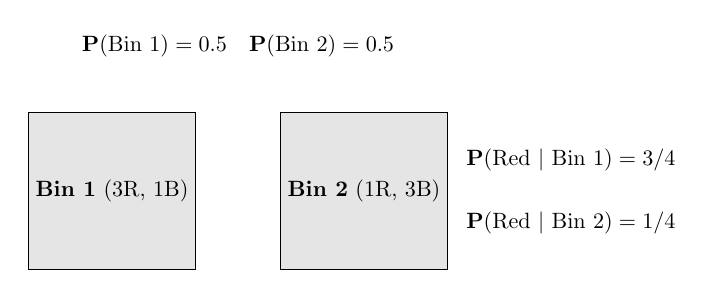
\begin{tikzpicture}[scale=0.8, transform shape, bin/.style={rectangle, draw, minimum width=2.5cm, minimum height=2.5cm, align=center}]
      
      \node[bin, fill=gray!20] (B1) at (0,0) {\textbf{Bin 1} (3R, 1B)};
      \node[bin, fill=gray!20] (B2) at (4,0) {\textbf{Bin 2} (1R, 3B)};

      % Likelihoods
      \node[anchor=west] at (5.5, 0.5) {$\mathbf{P(\text{Red } | \text{ Bin 1})} = 3/4$};
      \node[anchor=west] at (5.5, -0.5) {$\mathbf{P(\text{Red } | \text{ Bin 2})} = 1/4$};
      
      % Prior
      \node[anchor=south] at (2, 2) {$\mathbf{P(\text{Bin 1})} = 0.5 \quad \mathbf{P(\text{Bin 2})} = 0.5$};
      
    \end{tikzpicture}
  \end{center}

  \begin{alertblock}{The Result}
    $P(\text{Bin 1 } | \text{ Red}) = \frac{P(\text{Red } | \text{ Bin 1}) \cdot P(\text{Bin 1})}{P(\text{Red})} = \frac{(3/4) \cdot (1/2)}{1/2} = \mathbf{0.75}$
  \end{alertblock}

\end{frame}

% --- SLIDE 21: BREAKING IT DOWN: PRIOR, LIKELIHOOD, POSTERIOR ---
\begin{frame}
\frametitle{Breaking It Down: Prior, Likelihood, Posterior}

  \begin{itemize}
    \item The power of the theorem lies in combining three distinct pieces of information to produce a single updated value.
    
    \item $\mathbf{P(H)}$ is the \textbf{Prior Probability} (or \textbf{Prior Belief}): Our initial probability of the hypothesis being true, *before* seeing the new evidence.
    
    \item $\mathbf{P(E|H)}$ is the \textbf{Likelihood}: The probability of seeing the evidence, *given* that the hypothesis is true. This is the new data.
    
    \item $\mathbf{P(H|E)}$ is the \textbf{Posterior Probability}: The updated probability of the hypothesis being true, *after* considering the new evidence.
  \end{itemize}

  % SPECIAL ELEMENT: Block to summarize the relationship
  \begin{block}{The Logic of the Update}
    The Posterior Probability is proportional to the Likelihood multiplied by the Prior.
    \begin{displaymath}
        \text{Updated Belief} \propto \text{New Evidence} \times \text{Old Belief}
    \end{displaymath}
  \end{block}

\end{frame}

% --- SLIDE 22: THE POWER OF "PRIOR BELIEF" ---
\begin{frame}
\frametitle{The Power of "Prior Belief"}

  \begin{itemize}
    \item The Prior Probability, $P(H)$, is the most philosophically challenging and important term in the Bayesian framework.
    
    \item If the Prior is extremely low (meaning the event is initially very unlikely), then strong evidence is required to overcome it.
    
    \item A highly subjective or incorrect Prior can lead to a flawed Posterior, regardless of the quality of the new evidence.
    
    \item The repeated application of Bayes' theorem causes the influence of the Prior to diminish over time as more evidence is incorporated.
  \end{itemize}

  % SPECIAL ELEMENT: Alert Block for philosophical importance
  \begin{alertblock}{The Subjectivity Challenge}
    A central critique of Bayesianism is that the Prior is often an educated guess (a "belief-type" probability), which introduces human subjectivity into the calculation.
  \end{alertblock}

\end{frame}



% --- SLIDE 24: WHY BAYES WAS "FORGOTTEN" (AND THEN "FOUND") ---
\begin{frame}
\frametitle{Why Bayes Was "Forgotten" (and then "Found")}

  \begin{itemize}
    \item Following its initial presentation, Bayes' Theorem was largely ignored for nearly 200 years, especially in scientific circles.
    
    \item The biggest reason was the computational difficulty: calculating the full theorem for complex, real-world problems was impossible without computers.
    
    \item Another reason was the philosophical objection to the \textbf{Prior Probability}, which many statisticians found too subjective for objective science.
    
    \item The \textbf{Bayesian Renaissance} occurred in the late 20th century due to powerful computers and the rise of Artificial Intelligence (AI) and complex data modeling.
  \end{itemize}

  % SPECIAL ELEMENT: Block summarizing modern utility
  \begin{block}{The Revival}
    Today, Bayesian methods are central to machine learning, personalized medicine, and large-scale data analysis, where updating beliefs with new data is key.
  \end{block}

\end{frame}


% --- SLIDE 25: CASE STUDY 2: THE MEDICAL TEST (THE PROBLEM) ---
\begin{frame}
\frametitle{Case Study 2: The Medical Test}

  \begin{itemize}
    \item This case study illustrates the power of Bayes' Theorem to correct our intuitive (and often wrong) understanding of conditional probability.
    
    \item \textbf{Scenario:} A rare disease affects 1 in 1,000 people. We have a test that is 99\% accurate.
    
    \item \textbf{Accuracy breakdown:} If you have the disease, the test is positive 99\% of the time (True Positive). If you are healthy, the test is negative 99\% of the time (True Negative).
    
    \item You, personally, take the test and receive a \textbf{positive result}. What is the actual probability that you have the disease?
  \end{itemize}

  % SPECIAL ELEMENT: Alert Block to emphasize the question
  \begin{alertblock}{The Intuitive Error}
    Most people intuitively guess "99\%" because the test is 99\% accurate. This ignores the extremely low \textbf{Prior Probability} of having the rare disease.
  \end{alertblock}

\end{frame}

% --- SLIDE 26: CASE STUDY 2: APPLYING BAYES' THEOREM ---
\begin{frame}
\frametitle{Case Study 2: The Medical Test (The Solution)}

  \begin{itemize}
    \item Let $H$ be the hypothesis (\textit{has the disease}) and $E$ be the evidence (\textit{test is positive}).
    
    \item \textbf{Prior Probability $P(H)$:} 1/1,000 or $0.001$.
    
    \item \textbf{Likelihood $P(E|H)$:} The True Positive rate: $0.99$.
    
    \item The calculation reveals that the probability of having the disease \textbf{given} a positive test, $P(H|E)$, is only about \textbf{9\%}.
  \end{itemize}

  % SPECIAL ELEMENT: Block with the calculation summary
  \begin{block}{The Full Calculation (Simplified)}
    The large number of \textbf{False Positives} (1\% of 999 healthy people) overwhelms the small number of True Positives (99\% of 1 sick person).
    \begin{itemize}
        \item For every 1,000 people: $\approx 1$ person is sick and tests positive.
        \item $\approx 10$ healthy people test positive (False Positives).
        \item Total positives: $1+10 = 11$. $P(\text{Sick } | \text{ Positive}) = 1/11 \approx \mathbf{9.01\%}$
    \end{itemize}
  \end{block}

\end{frame}

% --- SLIDE 27: DISCUSSION: THE POWER OF THE PRIOR ---
\begin{frame}
\frametitle{Discussion: The Power of the Prior}

  \begin{itemize}
    \scriptsize
    \item This case study demonstrates how an initially low \textbf{Prior Probability} can dramatically suppress a seemingly strong piece of \textbf{evidence}.
    
    \item The low base rate (the rarity of the disease) means that most positive results are actually \textbf{False Positives}.
    
    \item In logic and critical thinking, this concept is called the \textbf{Base Rate Fallacy}—the tendency to ignore the prior probability.
    
    \item This has critical implications for public health screening, legal evidence, and assessing claims about rare phenomena.
  \end{itemize}

  % SPECIAL ELEMENT: Nested List for discussion prompts
  \begin{block}{Questions}
      \begin{enumerate}
      \item If the disease were common (e.g., $P(H)=0.1$), how would the Posterior Probability change?
      \item Why is it so hard for the human brain to intuitively account for low base rates?
      \item What logical safeguard does Bayes' theorem provide against jumping to conclusions?
  \end{enumerate}
    
  \end{block}

\end{frame}


% --- SLIDE 28: THE RISE OF "STATISTICS": R.A. FISCHER ---
\begin{frame}
\frametitle{The Rise of "Statistics": R.A. Fischer}

  \begin{itemize}
    \item While Bayes was largely ignored, the 20th century saw the spectacular rise of \textbf{Frequentist Statistics}, largely guided by \textbf{Sir Ronald Aylmer Fischer} (1890–1962).
    
    \item Fischer developed the core mathematical tools used in modern science, including the design of experiments and the analysis of variance (ANOVA).
    
    \item He argued strongly for an objective approach, rejecting the use of subjective \textbf{Prior Probabilities} inherent in the Bayesian framework.
    
    \item Fischer's work provided a clear, repeatable, and non-subjective method for drawing conclusions from data.
  \end{itemize}

  % SPECIAL ELEMENT: Block for Context
  \begin{block}{Science and Objectivity}
    Fischer's methods were rapidly adopted because they provided a rigorous, step-by-step procedure for proving scientific claims that appeared to be free of personal belief.
  \end{block}

\end{frame}

% --- SLIDE 29: THE FREQUENTIST VIEW: PROBABILITY AS LONG-RUN FREQUENCY ---
\begin{frame}
\frametitle{The Frequentist View: Probability as Long-Run Frequency}

  \begin{itemize}
    \item For a \textbf{Frequentist}, probability is defined solely by the long-run outcome of a repeatable process.
    
    \item They do not assign probabilities to hypotheses or causes; a hypothesis is either true or false, not "75\% probable."
    
    \item Instead, they focus on the probability of the \textbf{data} observed, assuming a certain hypothesis (the null) is true.
    
    \item This perspective provides the foundation for statistical tools like confidence intervals and hypothesis testing.
  \end{itemize}

  % SPECIAL ELEMENT: Simple definition
  \begin{itemize}
      \item \textbf{Key Idea:} A Frequentist probability is what you would measure if you could repeat an experiment an infinite number of times.
  \end{itemize}

\end{frame}

% --- SLIDE 30: FISCHER'S BIG IDEA: THE NULL HYPOTHESIS ---
\begin{frame}
\frametitle{Fischer's Big Idea: The Null Hypothesis}

  \begin{itemize}
    \item Fischer formalized the method of \textbf{Null Hypothesis Significance Testing} (NHST), the dominant paradigm in science for decades.
    
    \item The \textbf{Null Hypothesis} ($H_0$) is a statement of no effect, no difference, or no change (e.g., Drug A has the same effect as a placebo).
    
    \item The goal of the experiment is not to prove the alternative, but to gather enough evidence to \textbf{reject} the null hypothesis.
    
    \item If we can show that the observed data is extremely unlikely under $H_0$, then we reject $H_0$ and conclude a significant effect exists.
  \end{itemize}

  % SPECIAL ELEMENT: Alert Block for the logical process
  \begin{alertblock}{The Logic of Proof}
    Frequentist logic is based on \textit{reductio ad absurdum}: if the assumption of "no effect" leads to a highly improbable observation, the assumption must be wrong.
  \end{alertblock}

\end{frame}

% --- SLIDE 31: THE FAMOUS "P-VALUE" EXPLAINED ---
\begin{frame}
\frametitle{The Famous "p-value" Explained}

  \begin{itemize}
    \item The result of NHST is the **p-value**, the most ubiquitous and often misunderstood number in modern science.
    
    \item The \textbf{p-value} is the probability of observing data \textit{as extreme as}, or more extreme than, what was actually observed, \textit{assuming the Null Hypothesis is true}.
    
    \item If the p-value is very small (typically less than $0.05$ or $5\%$), we reject $H_0$ and declare the result \textbf{statistically significant}.
    
    \item Crucially, the p-value \textbf{is not} the probability that the null hypothesis is false, nor is it the probability that the finding is true.
  \end{itemize}

  % SPECIAL ELEMENT: Simple equation showing the definition
  \begin{equation*}
    p\text{-value} = P(\text{Data or more extreme} \mid H_0 \text{ is true})
  \end{equation*}

\end{frame}

% --- SLIDE 32: WHAT "STATISTICALLY SIGNIFICANT" REALLY MEANS ---
\begin{frame}
\frametitle{What "Statistically Significant" Really Means}

  \begin{itemize}
    \item When a result is declared \textbf{statistically significant}, it means the p-value is below the pre-set threshold (usually $\alpha=0.05$).
    
    \item Logically, it means the observed data is so unlikely under the assumption of no effect (the Null Hypothesis) that we must conclude the Null is false.
    
    \item It \textbf{does not} mean the effect is large, important, or even true with 95\% certainty.
    
    \item The phrase simply indicates that a difference was observed that is unlikely to be due purely to random chance.
  \end{itemize}

  % SPECIAL ELEMENT: Block to clarify a common misconception
  \begin{block}{A Common Mistake}
    A small p-value does \textbf{not} mean $P(\text{Null is True}) < 0.05$. It is a conditional statement about the data, not the hypothesis.
  \end{block}

\end{frame}

% --- SLIDE 33 (NEW): P-VALUE EXAMPLE: DRUG EFFICACY ---
\begin{frame}
\frametitle{P-Value Example: Drug Efficacy}

  \begin{itemize}
    \item \textbf{Scenario:} A new drug is tested against a placebo for an illness. We want to know if the drug actually works.
    
    \item \textbf{Null Hypothesis ($\mathbf{H_0}$):} The new drug has *no different* effect than the placebo. Any difference is due to chance.
    
    \item After the trial, we find the drug group recovered 10\% faster than the placebo group.
    
    \item The statistical test yields a $\mathbf{p\text{-value} = 0.03}$ (or 3\%).
  \end{itemize}

  % SPECIAL ELEMENT: Alert Block to interpret the p-value
  \begin{alertblock}{Interpretation}
    A $p=0.03$ means: if the drug truly did nothing (if $H_0$ were true), there would only be a 3\% chance of seeing a result this extreme or better. Since 3\% is less than our 5\% cutoff, we \textbf{reject the Null Hypothesis} and conclude the drug has a statistically significant effect.
  \end{alertblock}

\end{frame}

% --- SLIDE 34 (SHIFTED): APPLICATION: THE RANDOMIZED CONTROLLED TRIAL (RCT) ---
\begin{frame}
\frametitle{Application: The Randomized Controlled Trial (RCT)}

  \begin{itemize}
    \item Fischer's frequentist framework is the basis for the gold standard of scientific evidence: the \textbf{Randomized Controlled Trial} (RCT).
    
    \item In an RCT, subjects are randomly assigned to a treatment group or a control (placebo) group to ensure fair comparison.
    
    \item The Null Hypothesis ($H_0$) states that the effect observed in both groups is the same (i.e., the drug does not work).
    
    \item The statistics calculate the probability (the p-value) that the observed difference between the groups could have happened just by chance.
  \end{itemize}

  % SPECIAL ELEMENT: Simple illustration of a randomized trial setup
  \begin{center}
    \textbf{Null Hypothesis} ($H_0$): $\text{Drug Effect} = \text{Placebo Effect}$
  \end{center}
  \begin{enumerate}
      \item Randomly assign subjects.
      \item Collect data on outcomes.
      \item Calculate $p$-value. If $p < 0.05$, reject $H_0$.
  \end{enumerate}

\end{frame}

% Continue from the previous document setup...

% --- SLIDE 37 (REVISED): ETHICAL MISUSE: FISCHER, SMOKING, AND RACE SCIENCE ---
\begin{frame}
\frametitle{Ethical Misuse: Fischer, Smoking, and Race Science}

  \begin{itemize}
    \item Sir Ronald A. Fischer himself actively employed statistical arguments to oppose the emerging consensus on health issues.
    
    \item \textbf{Smoking:} Fischer claimed the correlation between smoking and lung cancer was likely due to a \textbf{confounding factor} (a common genetic predisposition to both smoking and cancer).
    
    \item His statistical authority and staunch refusal to accept non-experimental evidence helped tobacco companies cast doubt on causal links for years.
    
    \item \textbf{Eugenics:} Fischer was also a prominent eugenicist who used statistical methods, particularly those related to the analysis of variance (ANOVA), to support racist theories about intelligence and genetics.
  \end{itemize}

  % SPECIAL ELEMENT: Alert Block emphasizing the danger of selective data use
  \begin{alertblock}{The Danger of Statistical Authority}
    Fischer's history demonstrates that logical and statistical rigor can be weaponized. The misuse of Frequentist principles can obscure real-world risks and lend false authority to prejudice.
  \end{alertblock}

\end{frame}

% --- SLIDE 38 (REVISED): MISUSE 2: THE "REPLICATION CRISIS" (\textit{p}-HACKING) ---
\begin{frame}
\frametitle{Misuse 2: The "Replication Crisis" (\textit{p}-Hacking)}

  \begin{itemize}
    \item The pressure to publish "statistically significant" results ($p < 0.05$) has led to unethical practices that undermine scientific validity.
    
    \item \textbf{\textit{p}-Hacking} refers to manipulating research practices to force the $p$-value below the arbitrary significance threshold.
    
    \item This practice drastically inflates the number of \textbf{False Positives} (Type I Errors) published in scientific literature.
    
    \item A study of $p$-hacked findings showed that the average published $p$-value in some fields was inflated, contributing to a crisis of reproducibility.
  \end{itemize}

  % SPECIAL ELEMENT: Nested List of p-Hacking Examples (More Concrete)
  \begin{block}{Examples of Unethical \textit{p}-Hacking}
    \begin{itemize}
        \item \textbf{Cherry-Picking:} Testing 20 different variables, finding one with $p=0.04$, and only reporting that one.
        \item \textbf{Optional Stopping:} Checking the $p$-value repeatedly and stopping the experiment *only* when $p < 0.05$.
        \item \textbf{Data Dredging:} Removing outliers or certain demographic groups to achieve significance.
    \end{itemize}
  \end{block}

\end{frame}


% --- SLIDE 40 (REVISED): CASE STUDY 3: THE TYPICAL P-HACKED FINDING (The Problem) ---
\begin{frame}
\frametitle{Case Study 3: The Typical \textit{p}-Hacked Finding}

  \begin{itemize}
    \item This case study explores the ethical implications of the $p$-value crisis within Frequentist statistics.
    
    \item \textbf{Scenario:} A researcher studies the effect of "Feeling Hungry" on "Aggressive Driving" in 100 participants. They find no significant link (original $p=0.15$).
    
    \item They decide to re-run the analysis, but this time only including men (a new, smaller sample) and find $p=0.048$.
    
    \item They publish the $p=0.048$ finding without mentioning the original non-significant test or the change in the sample group.
  \end{itemize}

  % SPECIAL ELEMENT: Block to define the logical problem
  \begin{block}{The Logical Problem}
    By changing the sample and running multiple tests until a result is found, the researcher has violated the core logic of the Null Hypothesis, making the final $p$-value meaningless.
  \end{block}

\end{frame}

% --- SLIDE 41 (REVISED): DISCUSSION: THE ETHICS OF THE P-VALUE ---
\begin{frame}
\frametitle{Discussion: The Ethics of the \textit{p}-Value}

  \begin{itemize}
    \item This scenario highlights how easily statistical significance can be manufactured without a genuine underlying effect.
    
    \item The original assumption of the Null Hypothesis test—that the test is pre-specified and run only once—is broken.
    
    \item If the test had been pre-specified for only men, $p=0.048$ would be legitimate; running it \textit{after} seeing the non-significant result is problematic.
  \end{itemize}

  % SPECIAL ELEMENT: Nested List for discussion prompts
  \begin{block}{Discussion: Protecting Scientific Integrity}
    \begin{enumerate}
        \item Does the researcher have an ethical obligation to report the original $p=0.15$ result?
        \item What statistical solution (like a \textbf{Bayesian analysis}) might avoid this problem of subjective testing choices?
        \item If you are a journal editor, what logical flaws would you identify in the published paper?
    \end{enumerate}
  \end{block}

\end{frame}

% --- SLIDE 23: BAYESIAN VS. FREQUENTIST: A CORE PHILOSOPHICAL DEBATE ---
\begin{frame}
\frametitle{Bayesian vs. Frequentist: A Core Philosophical Debate}

  \begin{itemize}
    \item The two main schools of thought in probability offer fundamentally different answers to "What is probability?"
    
    \item The \textbf{Frequentist} view: Probability is an objective property of the world—the long-run frequency of an event over repeated trials.
    
    \item The \textbf{Bayesian} view: Probability is a measure of subjective knowledge or degree of belief, which is updated as new evidence is processed.
    
    \item This philosophical split governs how research is designed, data is analyzed, and conclusions are drawn in science and industry.
  \end{itemize}

  % SPECIAL ELEMENT: Table Comparison
  \begin{table}
    \centering
    \caption{Key Differences}
    \begin{tabular}{lll}
      \toprule
      \textbf{Concept} & \textbf{Frequentist} & \textbf{Bayesian} \\
      \midrule
      Definition of $P$ & Long-run ratio (objective) & Degree of belief (subjective) \\
      Hypothesis & Is fixed (true or false) & Has a probability $P(H|E)$ \\
      Data Role & To test the null hypothesis & To update the prior belief \\
      \bottomrule
    \end{tabular}
  \end{table}

\end{frame}


% --- SLIDE 42 (SHIFTED): PROBABILITY IN THE 21ST CENTURY: BIG DATA ---
\begin{frame}
\frametitle{Probability in the 21\textsuperscript{st} Century: Big Data}

  \begin{itemize}
    \item The explosion of digital data has cemented the role of probability as a foundational logic in the modern world.
    
    \item Traditional Frequentist methods struggle with the complexity, volume, and structure of modern data sets (e.g., streaming data, network graphs).
    
    \item \textbf{Bayesian methods} have surged in popularity because they naturally handle sequential decision-making and incorporating prior knowledge at a massive scale.
    
    \item Every prediction, classification, and recommendation made by digital systems is essentially a probabilistic calculation.
  \end{itemize}

  % SPECIAL ELEMENT: Block summarizing the shift
  \begin{block}{From Coin Flips to Cloud Computing}
    The philosophical battle between Bayes and Fischer is largely over: in the world of big data and AI, the Bayesian framework for belief updating has proved uniquely powerful.
  \end{block}

\end{frame}

% --- SLIDE 43 (SHIFTED): APPLICATION 1: HOW SPAM FILTERS "THINK" ---
\begin{frame}
\frametitle{Application 1: How Spam Filters "Think"}

  \begin{itemize}
    \item One of the earliest and most common applications of Bayesian logic is the \textbf{Naive Bayes Classifier} used in spam filters.
    
    \item The filter calculates $P(\text{Spam } | \text{ Word})$ for every word in an email, which is the probability the email is spam \textit{given} a specific word is present.
    
    \item It uses a historical \textbf{Prior Probability} based on the overall frequency of spam in your inbox.
    
    \item The final decision is a combination of these probabilities, updating its "belief" that an email is spam based on its content.
  \end{itemize}

  % SPECIAL ELEMENT: Simple formula highlighting the core calculation
  \begin{displaymath}
    P(\text{Spam} \mid \text{Word}) \propto P(\text{Word} \mid \text{Spam}) \times P(\text{Spam})
  \end{displaymath}

\end{frame}

% Continue from the previous document setup...

% --- SLIDE 44 (SHIFTED): APPLICATION 2: HOW NETFLIX RECOMMENDS MOVIES ---
\begin{frame}
\frametitle{Application 2: How Netflix Recommends Movies}

  \begin{itemize}
    \item Recommendation systems, like those used by Netflix or Amazon, are built on the logic of \textbf{probabilistic matrices}.
    
    \item The system calculates the probability that a user will like a given item, based on how similar users have rated it.
    
    \item This is often achieved using \textbf{Collaborative Filtering}, which predicts a missing rating by analyzing a large network of user preferences.
    
    \item Every movie or product displayed to you is a high-probability prediction that maximizes your expected enjoyment (utility) for the platform.
  \end{itemize}

  % SPECIAL ELEMENT: Nested List to show the data points
  \begin{block}{The Probabilistic Data Points}
    \begin{itemize}
        \item $P(\text{User A likes Movie X } | \text{ User A liked Movie Y})$
        \item $P(\text{User A is similar to User B})$
        \item $P(\text{User A will click this title})$
    \end{itemize}
  \end{block}

\end{frame}

% --- SLIDE 45 (SHIFTED): THE LOGIC OF RISK: INSURANCE, FINANCE, AND WEATHER ---
\begin{frame}
\frametitle{The Logic of Risk: Insurance, Finance, and Weather}

  \begin{itemize}
    \item Probability is the foundational language of any industry that deals with future uncertainty.
    
    \item \textit{Insurance} relies on calculating the probability of a specific event (fire, accident, death) to set premiums and mitigate risk.
    
    \item \textit{Finance} uses sophisticated probabilistic models (e.g., Value at Risk or VaR) to predict the likelihood of large market losses.
    
    \item \textit{Weather Forecasting} is entirely probabilistic, estimating the chance of rain based on massive inputs of atmospheric data and historical patterns.
  \end{itemize}

  % SPECIAL ELEMENT: Block to define the professional role
  \begin{block}{Actuaries and Quantifying Risk}
    An \textbf{Actuary} is a business professional who deals with the measurement and management of risk and uncertainty using advanced statistical models. They are essential to the insurance industry.
  \end{block}

\end{frame}

% --- SLIDE 46 (SHIFTED): ARTIFICIAL INTELLIGENCE & MACHINE LEARNING ---
\begin{frame}
\frametitle{Artificial Intelligence \& Machine Learning}

  \begin{itemize}
    \item Nearly all modern \textbf{Artificial Intelligence} (AI) is based on statistical, rather than purely deterministic, models.
    
    \item \textbf{Machine Learning} (ML) works by iteratively adjusting the probabilities assigned to connections within a network based on training data.
    
    \item A self-driving car, for instance, is not "sure" a pedestrian is a person; it calculates a high probability (e.g., $P(\text{Person})=0.999$).
    
    \item AI decisions are rarely binary (Yes/No); they are calculated degrees of certainty, making probability the core of intelligence.
  \end{itemize}

  % SPECIAL ELEMENT: Simple definition
  \begin{itemize}
      \item \textbf{Key Idea:} AI teaches computers to make the most probable decision, not the certain decision, given the available information.
  \end{itemize}

\end{frame}

% --- SLIDE 47 (SHIFTED): CASE STUDY 4: THE ETHICS OF ALGORITHMIC BIAS ---
\begin{frame}
\frametitle{Case Study 4: The Ethics of Algorithmic Bias}

  \begin{itemize}
    \item Algorithmic systems, built on historical data, can inadvertently perpetuate and amplify societal biases.
    
    \item \textbf{Scenario:} A probabilistic model is used by a bank to predict the credit risk of loan applicants based on historical data.
    
    \item If the historical data contains systemic biases against a certain demographic, the model will learn that $P(\text{Loan Default } | \text{ Demographic X})$ is artificially high.
    
    \item The model is mathematically sound, but its reliance on flawed prior data leads to ethically unjust, discriminatory decisions.
  \end{itemize}

  % SPECIAL ELEMENT: Alert Block for the central question
  \begin{alertblock}{The Logic of Bias}
    The bias in the outcome is the result of using a high-quality Likelihood ($P(\text{Data } | \text{ Default})$) and a strong, but flawed, historical Prior Probability ($P(\text{Default})$) for that group.
  \end{alertblock}

\end{frame}

% Continue from the previous document setup...

% --- SLIDE 48 (REVISED): DISCUSSION: THE ETHICS OF ALGORITHMIC BIAS ---
\begin{frame}
\frametitle{Discussion: The Ethics of Algorithmic Bias}

  \begin{itemize}
    \item The problem of bias reveals that the logic of probability is only as ethical as the data it is trained on.
    
    \item When a model calculates a high probability of risk for a protected group, it is often reflecting historical discrimination, not just future risk.
    
    \item This forces a logical choice: should we use the mathematically optimal model, or a model adjusted for fairness?
  \end{itemize}

  % SPECIAL ELEMENT: Nested List for discussion prompts
  \begin{block}{Discussion: Challenging Fair Probabilities}
    \begin{enumerate}
        \item If a model shows $P(\text{Default } | \text{ Group X})$ is high, is the model reflecting reality or reinforcing prejudice?
        \item How can we adjust the **Prior Probability** in an AI system to ensure a "fair start" for all groups?
        \item Is a system that optimizes for profit (mathematical probability) always in conflict with a system that optimizes for social justice?
    \end{enumerate}
  \end{block}

\end{frame}

% --- SLIDE 49 (REVISED): PROBABILITY AND THE LIMITS OF HUMAN PREDICTION ---
\begin{frame}
\frametitle{Probability and the Limits of Human Prediction}

  \begin{itemize}
    \item Despite the complexity of AI, predictive models often perform surprisingly poorly when forecasting long-term, specific human behavior or societal trends.
    
    \item \textbf{Simple models} (like assigning equal weight to a few key factors) often outperform both highly complex AI and human experts.
    \item This phenomenon, noted by statisticians like Robyn Dawes, suggests that our complex models often fall prey to \textbf{overfitting} noise in the data.
    \item Logically, the inclusion of too many factors introduces complexity that outweighs any predictive gain, leading to less reliable probabilities.
  \end{itemize}

  % SPECIAL ELEMENT: Block summarizing the finding
  \begin{block}{The Power of Simplicity}
    When predicting human outcomes (e.g., job success, relationshis, elections), a simple, transparent model based on probability can often achieve greater accuracy than a convoluted, black-box AI.
  \end{block}

\end{frame}

% --- SLIDE 50: FINAL THOUGHTS AND CONCLUSION (Concluding Slide) ---
\begin{frame}
\frametitle{Conclusion: From Pascal's Dice to AI's Logic}

  \begin{itemize}
    \item Probability emerged from simple games of chance but evolved into a powerful framework for human logic and scientific inquiry.
    
    \item The philosophical debate between \textbf{Frequentism} and \textbf{Bayesianism} reflects two distinct ways humans conceptualize and manage uncertainty.
    
    \item Today, probability forms the invisible architecture of the digital world, driving decision-making from finance to personalized medicine.
    
    \item Understanding the history and logic of probability is essential for evaluating evidence, recognizing bias, and mastering critical thinking in the modern age.
  \end{itemize}

  % SPECIAL ELEMENT: Thank you and final discussion prompts
  \begin{block}{Thank You \& Final Questions}
    \begin{itemize}
        \item Which school of probability (Frequentist or Bayesian) do you find more compelling for general life decisions, and why?
        \item How does the existence of "Black Swan" events challenge the very idea that all uncertainty is measurable?
    \end{itemize}
  \end{block}

\end{frame}

\end{document}